\section{Nichtlineare Gleichungssysteme}

\subsection{Funktionen mit mehreren Variablen}

auch multivariat gennant, hier nur skalarwertige Funktionen (keine Komplexen Zahlen). Definition:
\begin{description}
	\item[Explizite Darstellung] Funktionsgleichung ist nach einer variablen aufgelöst.
		$$y = f(x_1, x_2, ...,x_n)$$
	\item[Implizite Darstellung] nicht nach einer Variablen aufgelöst(nur n-1
		unabhängige Variablen)
		$$F(x_1, x_2, ..., x_n) = 0$$
\end{description}

für vektorwertige funktionen

$$\vec{f}(x_1, ..., x_n) =
	\begin{pmatrix}
		y_1 = f_1(x_1, ..., x_n) \\
		\hdots                   \\
		y_m = f_m(x_m, ..., x_m) \\
	\end{pmatrix}
$$


\subsubsection{Graphische Darstellungsformen}
Funktionen mit 2 Variablen können 3D dargestellt werden. \\
Interpretieren als $z = f(x, y)$

% TODO code
\begin{multicols}{2}
	\begin{description}
		\item[Fläche] Punkte $(x, y, f(x,y))$
			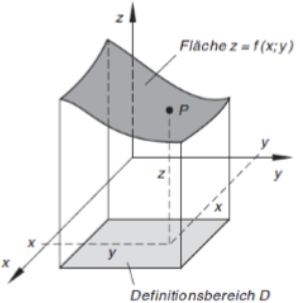
\includegraphics[width=0.95\linewidth]{nlinear-darstellung-flaeche}
		\item[Schnittkurve] bei konstanter Höhe $z$, auch Höhen-/Contour-Plot
			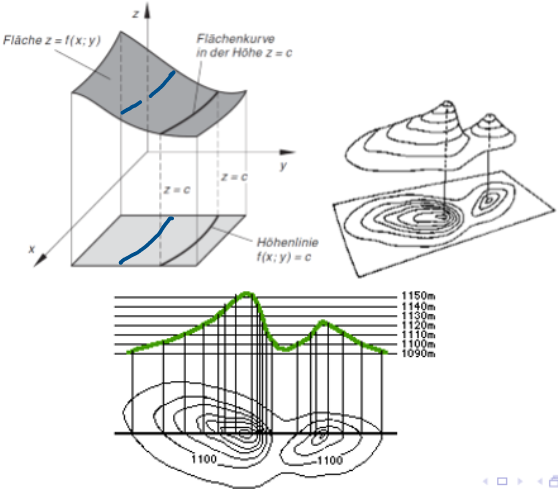
\includegraphics[width=0.95\linewidth]{nlinear-darstellung-schnitt}
	\end{description}
\end{multicols}



\subsection{Partielle Ableitungen}

Nur eine der Variablen wird abgeleitet, der Rest als Konstante behandelt.
Visuell entspricht dies der Steigung an einer Flächentangente. \vfill
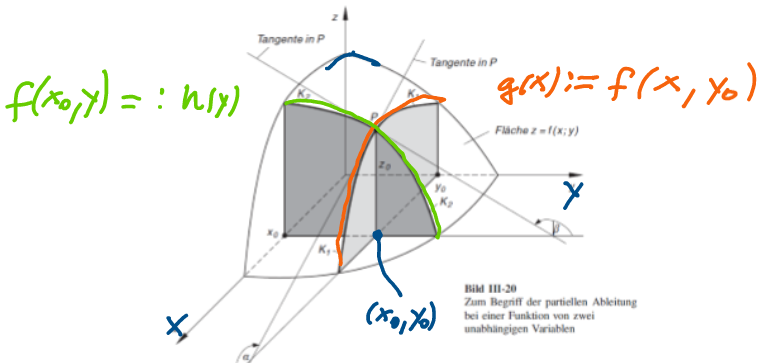
\includegraphics[width=0.95\linewidth]{partabl-vis}
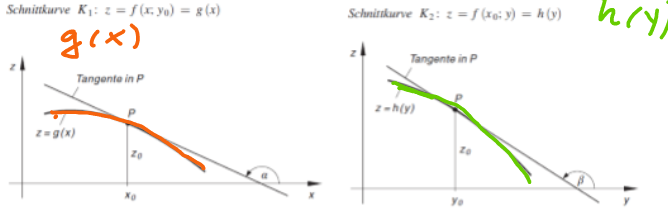
\includegraphics[width=0.95\linewidth]{partabl-vis-einzel}


\subsubsection{Partielle Ableitungen 1. Ordnung}
Beispiel nach x abgeleitet(normale Ableitungsregeln, andere Variablen als Konstanten
betrachten):
$$
	\frac{\partial f}{\partial x} =
	\lim \limits_{\Delta x \to 0} \frac{f(x + \Delta x, y) - f(x,y)}{\Delta x} \\

	\begin{align*}
		f(x, y)                       & = 3xy^3 + 10x^2y + 5y + 3y * sin(5xy) \\
		\frac{\partial f}{\partial x} & =
		3 * 1 * y^3 + 10 * 2x + 0 + 3y * cos(5xy) * 5 * 1 * y
	\end{align*}
$$

